\begin{frame}{Calcul le périmètre des figures suivantes.}
    \begin{minipage}{0.45\textwidth}
        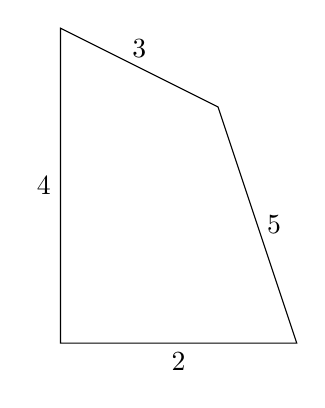
\begin{tikzpicture}
            \draw (0,0)-- node [midway, left] {4} (0,4)--node [midway,above]{3} (2,3) --node [midway, right]{5} (3,0) -- node [midway,below] {2} cycle;
        \end{tikzpicture}
    \end{minipage}
    \hfil
    \begin{minipage}{0.45\textwidth}
        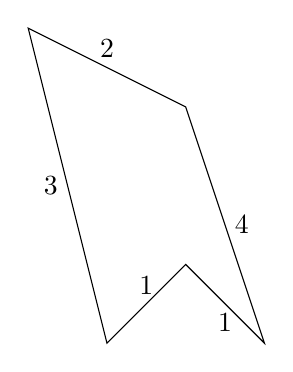
\begin{tikzpicture}
            \draw (1,0)-- node [midway, left] {3} (0,4)--node [midway,above]{2} (2,3) --node [midway, right]{4} (3,0) -- node [midway,below] {1} (2,1)-- node [midway,above]{1}cycle;
        \end{tikzpicture}
    \end{minipage}
\end{frame}

\begin{frame}{}
        \begin{minipage}{0.45\textwidth}
            Le périmètre du triangle est 20cm. Calculer AB
            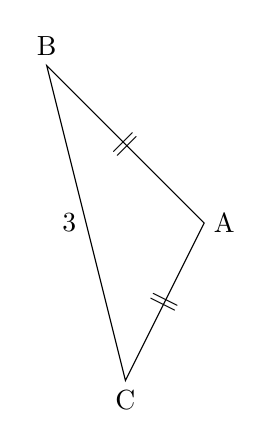
\begin{tikzpicture}
            \draw (1,0)node[below]{C}-- node [midway, left] {3} (0,4) node[above]{B}--node [midway,sloped]{$\parallel$} (2,2) node [right]{A} --  node [midway,sloped]{$\parallel$}cycle;
        \end{tikzpicture}
        \end{minipage}
        \hfil
        \vrule
        \hfil
        \begin{minipage}{0.45\textwidth}
            Le périmètre du quadrilatère est 119cm. Calculer AB
            \begin{tikzpicture}
            \draw (2,0)node[below]{C}-- node [midway, left] {31} (0,4) node[above]{B}--node [midway,sloped]{$\parallel$} (2,2) node [above]{A} --node [midway,sloped]{$\parallel$} (5,3) node [right]{D}--  node [midway,sloped]{$\parallel$}cycle;
        \end{tikzpicture}
        \end{minipage}
\end{frame}

\begin{frame}
    Paul, Émile et Victor ont eu un contrôle de maths. 
    \begin{itemize}
        \item À eux trois, leur moyenne est de 12.
        \item Paul a eu deux fois plus de points qu'Émile
        \item Victor a eu 4 points de moins qu'Émile
    \end{itemize}

    Quelle est la note de chacun ?
\end{frame}

\begin{frame}{Trouve le nombre}
    Je cherche un nombre tel que si : 
    \begin{itemize}
        \item Je le multiplie par 3.
        \item J'ajoute 4
        \item J'obtiens 37
    \end{itemize}
    \vspace*{0.5cm}
    \hrule
        Je cherche un nombre tel que le triple de ce nombre est égale à ce nombre auquel on ajoute 12.
\end{frame}